\chapter{Tecnología CMOS}\label{cap:tecnologia_cmos}

\section{Introducción}\label{cap:intro_cmos}

\paragraph{}
La tecnología CMOS, que es ampliamente utilizada en el diseño de circuitos integrados
en la actualidad, se basa en la posibilidad de integrar en un mismo substrato
semiconductores con ambos dopados (\textit{n} y \textit{p}). Con ello podemos implementar transistores
MOSFET tanto PMOS como NMOS en un mismo diseño.

\paragraph{}
Es una tecnología que cumple ya los
50 años, debido a que empezó a ponerse en práctica a mediados de los años 1960.
Inicialmente se usó principalmente en circuitos digitales, debido a que los
transistores CMOS solo consumen potencia cuando conmutan, a diferencia de los
transistores de unión bipolar. Por otra parte, es más sencillo disminuir su tamaño
y tienen un menor coste de fabricación.

\paragraph{}
Poco a poco se fue introduciendo la tecnología CMOS en el diseño de circuitos
analógicos. Los bajos costes y la posibilidad de crear circuitos digitales y
analógicos en el mismo chip hacían esta opción muy interesante. Pero aún así, los
transistores bipolares eran mucho menos ruidosos y más rápidos que los MOSFET, por
lo que la trancisión fue lenta. Con el desarrollo de la tecnología CMOS, la velocidad
y el ruido de éstos, se ha visto muy mejorada, y actualmente domina el mercado,
aunque en muchos casos se sigue usando tecnología bipolar.
% Mirar un poco más esto (Historia y actual uso de las tecnologías del silicio)


\section{Proceso de fabricación}\label{cap:fabricacion}

\paragraph{}
La gran mayoría de los circuitos integrados CMOS estan construidos sobre silicio.
El silicio (Si), elemento de número atómico 14, es muy abundante en la Tierra, aunque
no se encuentra de forma pura, sino como óxidos de silicio o silicatos. Entre los
óxidos de silicio, basados fundamentalmente en la sílice o dióxido de silicio
(SiO\textsubscript{2}), se encuentran el cuarzo y el sílex, ambos ampliamente extendidos
en la corteza terrestre. Los silicatos son sales basadas en el ión silicato (SiO\textsubscript{4}),
y forman parte de minereales como los feldespatos, micas, berilio.

{\huge\textbf{Leer algo en el libro de minerales y rocas en casa!!!!!!!!!}}

\paragraph{}
A pesar de estar en tan alta abundancia en la Tierra, como se dijo antes, el silicio
puro no se dá naturalmente, debe ser refinado y cristalizado. El proceso consiste,
tratado de manera sencilla, en extraer el óxigeno de los compuestos mencionados arriba
a base de añadir carbono y fundir la mezcla en un horno. Tras éste y otros porcesos
obtendríamos silicio relativamente puro, pero en forma policristalina (habitualmente
nos referiremos a éste como polisilicio). Esta forma contiene silicio puro, pero
cristalizado en pequeños cristales independientes con diferentes planos cristalinos
creando efectos de borde en el interior del conglomerado, que anulan los efectos
semiconductores del silicio.

\paragraph{}
Para construir un único monocristal de silicio se suele usar el llamado proceso
de Czochralski, en el cual, una varilla de silicio usada como semilla se va
rotando en un baño de silicio puro fundido a unos 1400\grad C de manera que va creciendo
en diámetro a medida que los átomos se silicio se van depositando en la capa externa.

\paragraph{}
Lo que queda es un lingote de aproximadamente un metro de largo y pocas decenas
de centímetro de diámetro de silicio monocristalino siguiendo la esctructura cristalina del
diamante.

\paragraph{}
Para ser usado en la industria de semiconductores, estos lingotes se deben laminar
en obleas de pocos milímetros de espesor sobre las que se implementarán los
circuitos integrados, que se suelen distribuir en una matriz ocupando toda la
superficie de la oblea que luego será cortada para separar cada "dado".

\paragraph{}
Con estos procesos tendríamos tan solo el substrato de silicio sobre el que
se debe construir el circuito, los transistores y otros dispositivos que se
necesiten. Esto se hace mediante fotolitografía, una técnica que crea permite
construir cada capa mediante la projección de una luz ultravioleta a través de
una máscara que permite o no pasar la luz según el layout diseñado.

\paragraph{}
Para empezar se recubre toda la oblea con un material fotosensible a la luz UV,
que dependiendo de si recibe luz o no, cambia sus propiedades haciendo que donde
ha recibido luz pueda ser eliminado posteriormente y quedar sólo donde no se recibió
luz, o viceversa. De esta forma obtenemos un recubrimiento selectivo con este
material, haciendo que, en un paso posterior podamos hacer crecer, sobre las zonas
sin recubrimiento, una capa de óxido de silicio si queremos un aislante, o de polisicio,
cuyos usos se tratarán más adelante, o de metal como condutor, habitualmente
aluminio o cobre, o algún tipo de dopado para crear las difusiones por ejemplo.

\paragraph{}
Tras las creación de cada capa, en la mayoría de los casos se realiza un pulido
fino de la superficie para que la siguiente capa asiente correctamente sobre una
superficie plana.

\section{Transistores CMOS}\label{cap:transistor_cmos}
\paragraph{}
El dispositivo fundamental que usa en cualquier circuito integrado CMOS es el
transistor CMOS, ya que es la base de funcionamiento de circuitos tanto digitales
(puertas lógicas, inversores, flip-flops, buffers), como de circuitos analógicos
(amplificadores operacionales y de transconductacia, convertidores analógico-digital,
referencias de tensión, bandgap).

\paragraph{}
El transistor CMOS es un dispositivo electrónico de 3 terminales que se basa
en una estructura MOS (Metal-Óxido-Semicondutor). En esta estructura, sobre un
substrato semicondutor se asienta una capa de Óxido aislante y sobre ella un
material metálico, que en las tecnologías actuales suele tratarse del polisilicio
que se mencionó anteriormente.

\paragraph{}
Usando la estructura vertical \textbf{M}etal-\textbf{Ó}xido-\textbf{S}emiconductor,
se puede construir un transistor creando a ambos lados de ella, zonas de silicio
altamente dopado donde contactaremos dos terminales, que llamaremos \textit{fuente} o \textbf{S}
(\textit{source}), y \textit{drenador} o \textbf{D} (\textit{drain}). En la capa superior
del polisilicio colocaremos el terminal llamado \textit{puerta} o \textbf{G} (\textit{gate}).
En la figura \ref{fig:nmos} podemos ver la estructura física de este dispositivo.


\paragraph{}
Cuando se aplica un voltage en puerta, el óxido crea un
condensador entre el polisilicio y el substrato semicondutor. De esta forma,
electrones presentes en substrato son atraídos hacia la superficie del substrato,
lo que facilita la creación de un canal, que permitirá la circulación de una
corriente entre las dos difusiones fuente y drenador. Cuando la tensión en la puerta
es menor que cierto valor, la creación del canal no se dá, y los terminales D y S
quedan electricamente aislados.

\paragraph{}
La dimensión de la puerta en la dirección que une drenador y fuente se llama
"longitud", notada como \textbf{L}. La otra dimensión de la puerta, perpendicular a ésta
se llama "anchura", abreviada como \textbf{W}

\paragraph{}
Como mencionamos al principio, también podemos crear transistores PMOS en estas
tecnologías. Esto se hace fabricándolos dentro de un pozo N, esto es, una zona
donde el substrato tipo-p original, se ha dopado de forma que se consigue un substrato
tipo-n. El transistor embebido en este pozo tiene, entonces, la misma estructura,
salvo que las difusiones para drenador y fuente son con dopado positivo \textbf{P+}.
Una representación de este tipo de transistor puede verse en la figura \ref{fig:pmos}.

\begin{figure}
	\centering
	\begin{subfigure}[b]{0.45\textwidth}
		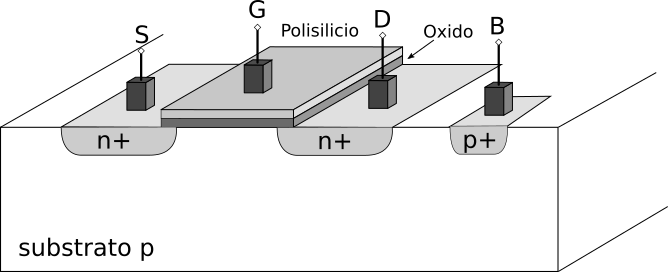
\includegraphics[width=\textwidth]{img/nmos.png}
		\caption{NMOS}
		\label{fig:nmos}
	\end{subfigure}
	~ %add desired spacing between images, e. g. ~, \quad, \qquad, \hfill etc.
	%(or a blank line to force the subfigure onto a new line)
	\begin{subfigure}[b]{0.45\textwidth}
		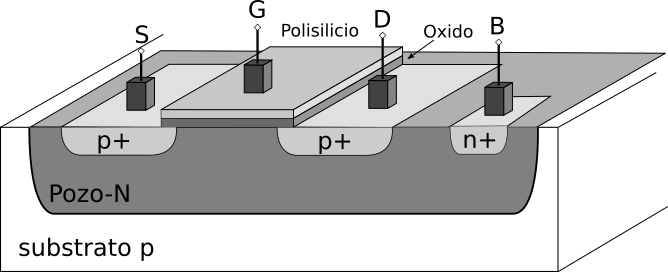
\includegraphics[width=\textwidth]{img/pmos.png}
		\caption{PMOS}
		\label{fig:pmos}
	\end{subfigure}
	\caption{Representación física de transistores MOS en tecnología CMOS}
	\label{fig:cmos_transistors}
\end{figure}

\section{Otros dispositivos en tecnología CMOS}\label{cap:otros_dispositivos}

\paragraph{}
Usando la misma tecnología es posible disponer en el mismo diseño otros dispositivos
además de los mencionados transistores.

\subsection{Diodos}\label{cap:diodos}
\paragraph{}
Una forma de crear diodos en esta tecnología es crear una zona de dopado N (difusión N+)
junto a una zona con dopado P (difusión P+).

\begin{figure}[h]
	\centering
	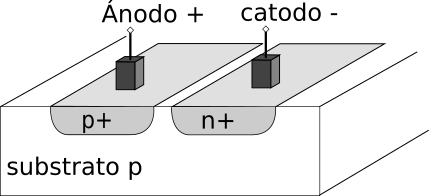
\includegraphics[width=0.4\textwidth]{img/diodo.png}
	\caption{Estructura física de un diodo de unión PN}
	\label{fig:diodo}
\end{figure}

\subsection{Transistores bipolares}\label{cap:bipolares}
\paragraph{}
También se pueden crear transistores de unión bipolar a partir de la creación
de dos uniones PN enfrentadas. En el caso de tener substrato P podemos conseguir
de forma sencilla un transistor tipo \textbf{PNP}, creando un contacto al susbtrato
P para el Colector (C), un pozo N dónde se crea un contacto a N+ para la base (B), y
una difusión positiva P+ dentro del pozo N, que funcionará como emisor (E).
Vease la siguiente imágen:

\begin{figure}[h]
	\centering
	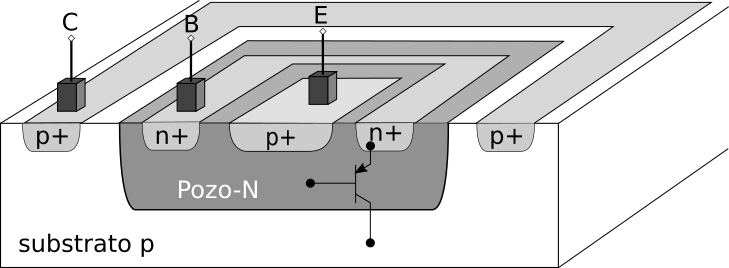
\includegraphics[width=0.7\textwidth]{img/pnp.png}
	\caption{Estructura física de un transistor de unión bipolar PNP}
	\label{fig:pnp}
\end{figure}

\paragraph{}
Crear un transistor NPN en una tecnología de susbtrato P es algo más complicado,
pero afortunadamente, existe la posibilidad de crear una estructura especial, que
va a ser muy usada en algunos casos con diferentes finalidades. Se trata del
llamado \textit{pozo N profundo} (\textit{Deep-N-Well} en inglés), que no
es más que un pozo N enterrado baja una capa de substrato P, que queda aislada del
substrato P del resto del chip si las uniones PN que forma con ambos substratos P,
están polarizadas inversamente.

\paragraph{}
De ésta forma podemos crear un transistor NPN entre el substrato profundo N,
colector (C), el substrato P encerrado por el anterior, base (B), y una difusión
N+ en el centro de este substrato P, que funcionará como emisor (E). Vease la
siguiente figura:

\begin{figure}[h]
	\centering
	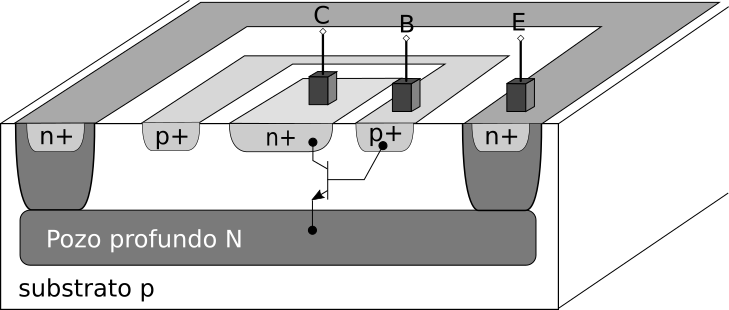
\includegraphics[width=0.7\textwidth]{img/npn.png}
	\caption{Estructura física de un transistor de unión bipolar NPN}
	\label{fig:npn}
\end{figure}


\section{Diseño de layout}

\paragraph{}
El término \textit{layout} hace referencia a la implementación física del circuito
electrónico que se quiere fabricar. El layout consiste en un dibujo con toda
la información que necesita la empresa fabricante para implementar el circuito
sobre la oblea de silicio. Dicha información se representa por medio de "capas"
que se distribuyen en un espacio bidimensional. Cada capa tiene un significado y
unas normas que cumplir. El trabajo del diseñador de layout es definir, dibujar y
verificar el layout de los diferentes bloques que componen el chip siguiendo
las normas dadas por el fabricante, y procurando el mejor funcionamiento posible
del circuito en el menor area que le sea posible.

Como veremos más adelante, el diseño del layout de un circuito afecta o puede afectar
mucho al funcionamiento final del mismo.

\subsection{Capas de layout}

\paragraph{}
Todo diseño de layout está compuesto de una cierta cantidad de capas, de las cuales
algunas tienen significado físico directo y otras son capas que usa el software de
diseño para verificaciones o para cambiar propiedades de otras capas.

\paragraph{NWELL}
Esta capa define el pozo N en una tecnología de substrato P. En ella se deben
situar los transistores PMOS y normalmente se polariza mediante difusiones \textbf{P+}
a la tensión más alta del circuito (VDD o similar).

\paragraph{WB}
Esta capa define el pozo enterrado (del inglés \textit{Well Buried}), o también
llamado pozo profundo (\textit{Deep-N-Well}), y como se introdujo en el capítulo
\ref{cap:bipolares}

\paragraph{XN}
Zona de difusión con dopado negativo N+, estará en las difusiones de drenador/fuente
de los transistores NMOS y en los contactos a substrato de los pozos N.

\paragraph{XP}
Zona de difusión con dopado positivo P+, de manera complementaria a la XN,
se usará para las difusiones de drenador/fuente
de los transistores PMOS y para los contactos al substrato P.

\paragraph{ACTIVE}
Zona activa

\paragraph{GC}
Zona donde se creará una capa de polisilicio (\textit{poly}). Si coincide con capa activa,
este posilicio creará puertas de transistores sobre una fina capa de óxido de silicio.
En los lugares donde no coincida con area activa se construirá sobre oxido grueso
de espesor no tan controlado y se usará para rutar líneas o para crear resistencias
de polisilicio por ejemplo.

\paragraph{CS}
Contacto. Normalmente son cuadrados que definen contactos entre el Metal 1 y el
polisilicio (si están sobre capa GC), o al substrato, si están sobre el substrato.

\paragraph{M1} Metal 1. Es el primero de los metales y se suele usar para contactar
transistores entre sí y con otros dispositivos, o para crear anillos de contactos
a substrato

\paragraph{M2-M3-...-(M5)} Otros metales. En función de la tecnología, pueden ser
más o menos capas de metal, por ejemplo 4 ó 6. La última capa de metal puede ser
diferente, ser más gruesa y menos resistiva. Habitualmente, para seguir un órden
y ayudar al rutado del circuito, se suele definir un criterio de direcciones
en función de si la capa de metal es par o impar se dispondrán horizontales o
verticales

\paragraph{V2-V3-...-(V5)} Vias. Crean conexiones verticales entre un metal y el
siguiente superior. Se suelen usar varios para cada conexión por evitar una
posible rotura y para disminuir la resistencia.

\subsection{Herramientas de CAD}

\paragraph{} Las herramientas de CAD (\textit{Computer Asisted Design}) se usan
en muchos campos de la ingeniería o la arquitectura, y actualmente, debido a la alta
complejidad de los diseños son de uso prácticamente obligado.

\paragraph{} En el caso que nos ocupa, el diseño de circuitos microelectrónicos,
tiene gran importancia el buen uso y conocimiento de las herramientas por parte de
diseñadores. En nuestro caso, estas técnicas tienen dos finalidades fundamentales:
el diseño y la simulación electrica y la implementación física. Entre ellas
hay muchas diferencias, pero también existe una inevitable relación de dependencia
entre ellas.

\paragraph{} Por otra parte, en microelectronica, debemos tener presente que
hay una división importante entre dos ámbitos que son bastante diferentes en cuanto
al flujo de diseño, simulación e implementación física, aunque ambos se basan sobre
la misma tecnología. Me refiero a la separación entre el ámbito \textbf{analógico}
y el \textbf{digital}.

\subsection{Problemas habituales en el diseño de layout}
